% Limbo: write-up for the Nexconn Build Challenge 2026.  Build: ./report/build.sh  (needs tectonic)
\documentclass[10pt,twocolumn]{article}

% ------------------------------------------------------------------ links (edit before final build)
\newcommand{\RepoURL}{https://github.com/kavyabhand/limbo}
\newcommand{\VideoURL}{https://youtu.be/bTRSKyyD-l0}
\newcommand{\LiveURL}{https://limbo-sooty.vercel.app}
\newcommand{\AppKey}{ik1qhw09iruvp}

% ------------------------------------------------------------------ packages
\usepackage[a4paper,margin=1.7cm,columnsep=0.65cm,top=1.8cm,bottom=1.9cm]{geometry}
\usepackage{libertinus}
\usepackage{amsmath}
\usepackage{graphicx}
\usepackage[table]{xcolor}
\usepackage{booktabs,tabularx,multirow,array}
\usepackage{tikz}
\usetikzlibrary{positioning,arrows.meta,fit,backgrounds,calc}
\usepackage{pgfplots}
\pgfplotsset{compat=1.18}
\usepackage[font=small,labelfont=bf,skip=4pt]{caption}
\usepackage{enumitem}
\usepackage{titlesec}
\usepackage{fancyhdr}
\usepackage{algorithm}
\usepackage[noend]{algpseudocode}
\usepackage{tcolorbox}
\usepackage{microtype}
\usepackage[colorlinks=true,linkcolor=accent,urlcolor=accent,citecolor=accent]{hyperref}
\hypersetup{pdftitle={Limbo: trip-keyed rooms for stranded travellers},pdfauthor={Team maxout},pdfsubject={Nexconn Build Challenge 2026}}

% ------------------------------------------------------------------ look
\definecolor{ink}{HTML}{111113}
\definecolor{ink2}{HTML}{52525B}
\definecolor{ink3}{HTML}{8A8A93}
\definecolor{line}{HTML}{E4E4E7}
\definecolor{subtle}{HTML}{F4F4F5}
\definecolor{accent}{HTML}{1D4ED8}
\definecolor{amber}{HTML}{B45309}
\definecolor{okgreen}{HTML}{15803D}
\definecolor{danger}{HTML}{B91C1C}
\color{ink}

\titleformat{\section}{\normalfont\large\bfseries}{\thesection}{0.6em}{}
\titleformat{\subsection}{\normalfont\normalsize\bfseries}{\thesubsection}{0.6em}{}
\titlespacing*{\section}{0pt}{1.1em}{0.45em}
\titlespacing*{\subsection}{0pt}{0.8em}{0.3em}
\setlist{nosep,leftmargin=1.2em}
\renewcommand{\arraystretch}{1.18}
\setlength{\aboverulesep}{0.3ex}\setlength{\belowrulesep}{0.4ex}

\pagestyle{fancy}
\fancyhf{}
\fancyhead[L]{\small\color{ink3}Limbo: trip-keyed rooms on the Nexconn Chat SDK}
\fancyhead[R]{\small\color{ink3}Team maxout}
\fancyfoot[C]{\small\color{ink3}\thepage}
\renewcommand{\headrulewidth}{0pt}

\newcommand{\shot}[1]{{\setlength{\fboxsep}{0pt}\setlength{\fboxrule}{0.4pt}\fcolorbox{line}{white}{\includegraphics[width=0.18\textwidth]{#1}}}}
\newcommand{\code}[1]{\texttt{\small #1}}
\newcommand{\stat}[2]{\begin{minipage}[t]{0.235\textwidth}\centering{\fontsize{22}{24}\selectfont\bfseries #1}\\[2pt]{\small\color{ink2}#2}\end{minipage}}

\begin{document}

% ------------------------------------------------------------------ title block
\twocolumn[{%
\begin{center}
  {\fontsize{24}{28}\selectfont\bfseries Limbo}\\[4pt]
  {\Large Trip-keyed rooms for stranded travellers, built on the Nexconn Chat SDK}\\[10pt]
  {\normalsize Team maxout}\\[2pt]
  {\small\color{ink2}Nexconn Build Challenge 2026 \,\textperiodcentered\, 14 November 2026}
\end{center}
\vspace{4pt}
\begin{tcolorbox}[colback=subtle,colframe=subtle,arc=4pt,left=10pt,right=10pt,top=6pt,bottom=6pt]
\small
\begin{tabularx}{\textwidth}{@{}l X l X@{}}
\textbf{Nexconn App Key} & \code{\AppKey} (Singapore data centre) & \textbf{Repository} & \href{\RepoURL}{\code{github.com/kavyabhand/limbo}} \\
\textbf{Demo video} & \href{\VideoURL}{\code{youtu.be/bTRSKyyD-l0}} \,(2:05) & \textbf{Live app} & \href{\LiveURL}{\code{limbo-sooty.vercel.app}} \\
\textbf{Built} & From scratch during the challenge (\S\ref{sec:before}) & \textbf{Licence} & MIT \\
\end{tabularx}
\end{tcolorbox}
\vspace{2pt}
\begin{center}
\stat{58/58}{end-to-end checks pass against a live Nexconn app}\hfill
\stat{30/30}{8-way races for one seat with exactly one winner}\hfill
\stat{94\,ms}{median server time to post a verified update}\hfill
\stat{0.8\,s}{median catch-up after a phone reconnects}
\end{center}
\vspace{6pt}
\begin{abstract}
\noindent When a flight is cancelled or a train stalls in fog, hundreds of people share the same problem and have no
way to reach each other. No one can create the group: strangers do not have each other's numbers, and the operator's
channels are one-way. We observe that a trip already has a public, shared key, its number and date, so a room for it
can exist \emph{before anyone joins}. Limbo maps every flight, train and bus to a Nexconn community channel that is
created on first visit; anyone who types the same trip number lands in the same room with no app and no sign-up.
Inside, a plain-language status line summarises crowd-confirmed facts scored by an explainable, decaying confidence
model; shared cabs and rooms let travellers split costs, with the last seat awarded to exactly one person under
contention; every message is translated into the reader's language; and verified staff can post official updates that
nobody else can forge. Because any channel member can write Nexconn message metadata, all live state is signed by the
server with Ed25519 and verified in every browser. We evaluate the system end to end against a live Nexconn app:
58 of 58 browser and API checks pass, 240 simultaneous seat claims across 30 trials produce exactly one winner every
time, and a phone that loses its connection catches up a median 0.8\,s after reconnecting.
\end{abstract}
\vspace{10pt}
}]

% ------------------------------------------------------------------ 1
\section{Introduction}
A disrupted trip produces the same questions from everyone on it: \emph{How late is it? Which desk is rebooking? Is
there a hotel? Is anyone sharing a cab into the city?} Answers exist, scattered across a gate announcement, a
departure board and the person who just walked back from the desk, but there is no channel connecting the people who
need them. Airline apps broadcast; social media is public and noisy; messaging groups need someone to create them and
everyone's phone number.

Limbo starts from a simple observation: \textbf{a trip number plus a date is a public key that everyone affected already
knows.} If a chat room is addressed by that key, it does not need an organiser or an invitation. The first person to
type \code{AI 101} opens it; the second is already in a room with the first.

\paragraph{Contributions.}
\begin{itemize}
  \item A \textbf{trip-keyed room} model on Nexconn community channels, created lazily and idempotently, with guest
        identities minted by the Server API so nobody signs up (\S\ref{sec:room}).
  \item A \textbf{crowd-confirmed board} with an explainable confidence score that scales with room size and decays
        with time, summarised in one status line (\S\ref{sec:board}).
  \item \textbf{Signed live state}: vote tallies and seat lists carried in Nexconn message metadata, signed with
        Ed25519 so edited or replayed state is rejected by every client (\S\ref{sec:trust}).
  \item \textbf{Fair shares}: shared cabs and rooms whose last seat goes to exactly one claimant, with a waitlist,
        automatic promotion and a private group channel per pool (\S\ref{sec:pools}).
  \item An \textbf{end-to-end evaluation} against a live Nexconn app, with no mocks (\S\ref{sec:eval}).
\end{itemize}

\begin{figure*}[t]
\centering
\shot{../assets/screens/01-landing.png}\hfill
\shot{../assets/screens/02-room-delay.png}\hfill
\shot{../assets/screens/03-chat-translated-pool.png}\hfill
\shot{../assets/screens/04-group-chat.png}\hfill
\shot{../assets/screens/05-room-cancelled-official.png}
\caption{Limbo on a phone: (1) type a trip number; (2) the room's status and board; (3) translated chat and a shared
room; (4) the private group for a shared room; (5) an official cancellation pinned for everyone.}
\label{fig:screens}
\end{figure*}

% ------------------------------------------------------------------ 2
\section{What existed before}\label{sec:before}
\paragraph{Prior tools.} Operator apps and SMS alerts are one-way and per-booking; they cannot connect passengers to
each other. Flight trackers show status but not what is happening at the gate. Public social media mixes millions of
trips and exposes identities. Messaging groups are the closest fit but require an organiser, phone numbers and an
invitation chain that never forms among strangers. None of these offer a shared space that exists by default for
everyone on a given trip.

\paragraph{This project.} Every line of code, design and copy in the repository was written during the challenge,
starting on 13 November 2026. Before that there was only the idea and a written product specification; no code,
design or earlier application.

% ------------------------------------------------------------------ 3
\section{System design}\label{sec:room}
\subsection{Rooms that exist before anyone joins}
A trip is normalised into a mode $m\in\{f,t,b\}$ (flight, train, bus), an upper-cased code $c$ and a date $d$. The
room is the Nexconn community channel
\begin{equation}
  \textit{channelId} = \texttt{lb}\,\Vert\, m \,\Vert\, c \,\Vert\, d_{\texttt{yyyymmdd}},
\end{equation}
for example \code{lbfAI10120261114}. The server creates the channel on the first visit and joins each visitor. We
probed the live API before relying on it: \code{create} succeeds when the channel already exists and \code{join}
succeeds for existing members, so two people opening a brand-new room simultaneously cannot break it. Because
\code{join} also succeeds on a channel that does not exist, Postgres records which rooms have been created. Dates are
limited to a window around today, and unrecognised codes ask for confirmation, which keeps typos from fragmenting a
trip.

\subsection{Guests with no sign-up}
A visitor receives an HMAC-signed, \code{SameSite=Lax} cookie holding a random 20-character guest ID and a generated
pseudonym (``Quiet Heron''). On each session the server mints a Nexconn access token through the Server API; the App
Secret never leaves the server, and tokens are not stored.

\subsection{Architecture}
Limbo has no WebSocket server of its own (Figure~\ref{fig:arch}). Browsers connect directly to Nexconn with the Web
SDK for chat, history, live metadata and translation. Anything that must be trusted (facts, votes, pools, official
updates) goes through Limbo's API, which validates it, records it in Postgres as the source of truth, and sends it to
Nexconn on the author's behalf as a custom message with signed metadata. Table~\ref{tab:nexconn} lists every Nexconn
capability used.

\begin{figure}[t]
\centering
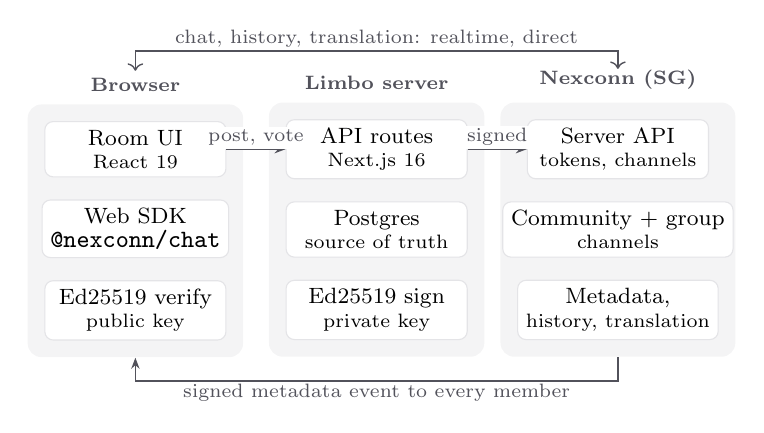
\begin{tikzpicture}[
  font=\footnotesize,
  box/.style={draw=line,fill=white,rounded corners=3pt,align=center,minimum width=2.3cm,minimum height=0.62cm,inner sep=3pt},
  grp/.style={draw=none,fill=subtle,rounded corners=5pt,inner sep=6pt},
  lab/.style={font=\scriptsize\bfseries,text=ink2},
  arr/.style={-{Stealth[length=4pt]},draw=ink2,line width=0.5pt},
  note/.style={font=\scriptsize,text=ink2,fill=white,inner sep=1pt}]
  % browser
  \node[box] (ui) {Room UI\\[-1pt]{\scriptsize React 19}};
  \node[box,below=0.28cm of ui] (sdk) {Web SDK\\[-1pt]{\scriptsize \code{@nexconn/chat}}};
  \node[box,below=0.28cm of sdk] (ver) {Ed25519 verify\\[-1pt]{\scriptsize public key}};
  % server
  \node[box,right=0.75cm of ui] (api) {API routes\\[-1pt]{\scriptsize Next.js 16}};
  \node[box,below=0.28cm of api] (pg) {Postgres\\[-1pt]{\scriptsize source of truth}};
  \node[box,below=0.28cm of pg] (sign) {Ed25519 sign\\[-1pt]{\scriptsize private key}};
  % nexconn
  \node[box,right=0.75cm of api] (sapi) {Server API\\[-1pt]{\scriptsize tokens, channels}};
  \node[box,below=0.28cm of sapi] (cc) {Community + group\\[-1pt]{\scriptsize channels}};
  \node[box,below=0.28cm of cc] (meta) {Metadata,\\[-1pt]{\scriptsize history, translation}};
  \begin{scope}[on background layer]
    \node[grp,fit=(ui)(ver)] (gb) {};
    \node[grp,fit=(api)(sign)] (gs) {};
    \node[grp,fit=(sapi)(meta)] (gn) {};
  \end{scope}
  \node[lab,above=1pt of gb] {Browser};
  \node[lab,above=1pt of gs] {Limbo server};
  \node[lab,above=1pt of gn] {Nexconn (SG)};
  \draw[arr] (ui) -- node[note,above]{post, vote} (api);
  \draw[arr] (api) -- node[note,above]{signed} (sapi);
  \draw[arr,<->] ($(gb.north)+(0,0.42)$) -- ++(0,0.25) -| node[note,pos=0.25,above]{chat, history, translation: realtime, direct} ($(gn.north)+(0,0.42)$);
  \draw[arr] (gn.south) -- ++(0,-0.3) -| node[note,pos=0.25,below]{signed metadata event to every member} (gb.south);
\end{tikzpicture}
\caption{Limbo's architecture. Chat flows directly between browsers and Nexconn; trusted state is written by the
server, signed, and delivered as message metadata to every client, which verifies it before display.}
\label{fig:arch}
\end{figure}

\begin{table*}[t]
\centering\small
\caption{How each feature maps to Nexconn. Every message, live tally and seat list travels through Nexconn.}
\label{tab:nexconn}
\begin{tabularx}{\textwidth}{@{}>{\raggedright\arraybackslash}p{4.1cm} >{\raggedright\arraybackslash}p{5.6cm} X@{}}
\toprule
\textbf{Feature} & \textbf{Nexconn capability} & \textbf{Detail} \\
\midrule
One room per trip, up to 10{,}000 people & Community channel (\code{/v4/community-channel/create}, \code{join}) & Created lazily and idempotently on first visit \\
No sign-up & Server API \code{/v4/auth/access-token/issue} & Token per session for a random guest ID; App Secret stays on the server \\
Updates, shared rides, notices & Custom messages \code{Limbo:Intel}, \code{Limbo:Pool}, \code{Limbo:Notice} & Registered before connect; sent by the server as the author, with \code{hasMetadata} \\
Live vote counts and seat lists & Message metadata (\code{metadata/set}; \code{onCommunityChannelMessageMetadataChanged}) & Every state change is signed (\S\ref{sec:trust}) and pushed to all clients in about a second \\
Private chat per shared cab or room & Group channel (\code{create}, \code{join}, \code{leave}, \code{joinPerm: 3}) & Members join only by winning a seat \\
Latecomers see what happened & History (\code{createMessagesQuery}, \code{loadNextPage}) & Also used to catch up after a reconnect \\
Everyone reads their own language & Built-in translation (\code{translateMessages}, \code{TranslateHandler}) & Per-device cache, length and age limits to protect the quota \\
Chat & Text messages via \code{CommunitySubChannel.sendMessage} & Sender's name, colour and language carried with each message \\
Connection state & \code{ConnectionStatusHandler} plus browser \code{online}/\code{offline} events & Offline notice and immediate catch-up on reconnect \\
\bottomrule
\end{tabularx}
\end{table*}

% ------------------------------------------------------------------ 4
\section{The board: crowd-confirmed facts}\label{sec:board}
Anyone can post a short fact of a given kind (delay, cancellation, gate change, rebooking desk, food, refund, safety).
Others confirm or dispute it with one tap. Each card's confidence is deliberately simple enough to explain in a
sentence:
\begin{align}
  r &= n_{\text{confirm}} - 1.25\, n_{\text{dispute}}, \\
  s(t) &= \max\!\left(0,\; r \cdot 2^{-\Delta t / h_k}\right),
\end{align}
where $\Delta t$ is the time since the last confirmation and $h_k$ the half-life for the card's kind (30\,min for a gate
change, 45\,min for a delay, 60\,min for a desk, up to 6\,h for a cancellation). A card is \emph{likely} once
$s \ge \tau_\ell$ and \emph{confirmed} once $s \ge \tau_c$, with thresholds that grow with the room so a room of three is
not stuck with an empty board (Table~\ref{tab:thr}). Weightier kinds (cancellation, rebooking, refund) multiply the
bar by 1.5. A card is \emph{contested} when enough people have voted and disputes exceed 60\% of confirmations.
Official updates bypass scoring and are pinned first. Figure~\ref{fig:decay} shows how stale confirmations fade.

\begin{table}[h]
\centering\small
\caption{Status thresholds by room size (base kinds).}
\label{tab:thr}
\begin{tabular}{@{}lcc@{}}
\toprule
\textbf{People in room} & \textbf{Likely} $\tau_\ell$ & \textbf{Confirmed} $\tau_c$ \\
\midrule
up to 5 & 1 & 2 \\
6--25 & 1.5 & 3 \\
more than 25 & 1.5 & 4 \\
\bottomrule
\end{tabular}
\end{table}

\begin{figure}[t]
\centering
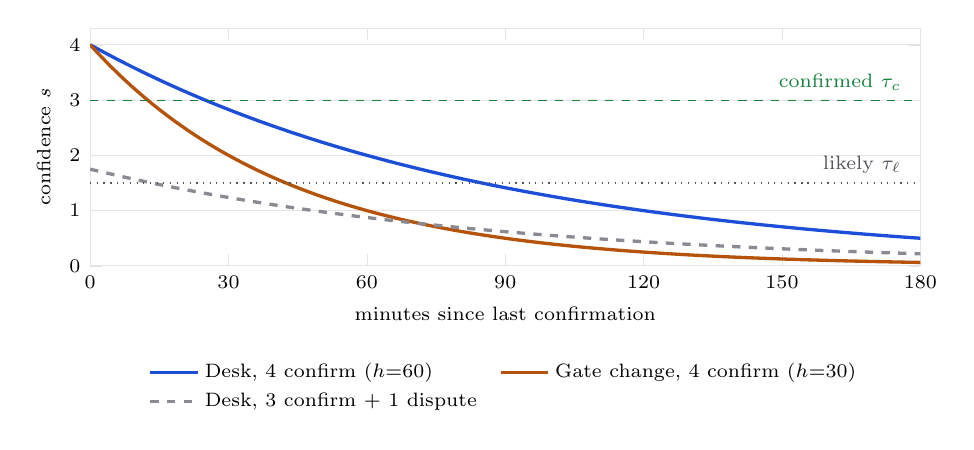
\begin{tikzpicture}
\begin{axis}[
  width=\columnwidth, height=4.6cm,
  xmin=0, xmax=180, ymin=0, ymax=4.3,
  xlabel={minutes since last confirmation}, ylabel={confidence $s$},
  xtick={0,30,60,90,120,150,180}, ytick={0,1,2,3,4},
  tick label style={font=\scriptsize}, label style={font=\scriptsize},
  axis line style={line}, tick style={line}, major grid style={line},
  ymajorgrids, legend style={font=\scriptsize,draw=none,at={(0.5,-0.36)},anchor=north,legend columns=2,/tikz/every even column/.append style={column sep=6pt}},
  legend cell align=left, samples=120, domain=0:180]
  \addplot[very thick,accent] {4*0.5^(x/60)};
  \addlegendentry{Desk, 4 confirm ($h{=}60$)}
  \addplot[very thick,amber] {4*0.5^(x/30)};
  \addlegendentry{Gate change, 4 confirm ($h{=}30$)}
  \addplot[very thick,ink3,dashed] {max(0,(3-1.25)*0.5^(x/60))};
  \addlegendentry{Desk, 3 confirm + 1 dispute}
  \addplot[okgreen,thin,dashed,domain=0:180] {3};
  \addplot[ink2,thin,dotted,domain=0:180] {1.5};
  \node[font=\scriptsize,okgreen,anchor=south east] at (axis cs:178,3) {confirmed $\tau_c$};
  \node[font=\scriptsize,ink2,anchor=south east] at (axis cs:178,1.5) {likely $\tau_\ell$};
\end{axis}
\end{tikzpicture}
\caption{Confidence decay for a room of 6--25 people. A desk confirmed by four people stays \emph{confirmed} for
25\,minutes and \emph{likely} for an hour unless someone reconfirms it; gate changes fade twice as fast.}
\label{fig:decay}
\end{figure}

The \textbf{status line} at the top of every room turns the board into one sentence: the strongest delay or
cancellation, its detail and its basis (``Delayed about 2 hours \textperiodcentered{} Confirmed by 4 people'',
``Official update from Demo Airlines''). A newer delay estimate supersedes an older one, so the line never shows two
contradicting numbers.

% ------------------------------------------------------------------ 5
\section{Trust}\label{sec:trust}
\paragraph{Signed metadata.} Live tallies ride on Nexconn message metadata, which is what lets every screen update in
about a second. But \code{message.setMetadata()} is available to any member of a community channel, so a visitor
could rewrite ``Confirmed by 3'' as ``Confirmed by 300''. Limbo therefore treats metadata as untrusted transport. The
server signs each state with a key only it holds,
\begin{equation}
  \sigma = \mathrm{Ed25519}_{sk}\!\left(\textit{cardId} \,\Vert\, \texttt{"|"} \,\Vert\, \textit{stateJSON}\right),
\end{equation}
and stores $\sigma$ beside the state. Every browser verifies with the public key it received at session start.
Edited state fails verification; genuine state copied onto another card fails too, because the card ID is part of
the signed message. Cards without a valid signature are never shown. Verification costs 0.83\,ms per card and signing
0.21\,ms (pure JavaScript \code{@noble/ed25519}); we moved off WebCrypto's Ed25519 after our browser tests showed it is
missing before Chrome~137, which silently hid every card on older phones.

\paragraph{Official means official.} Staff are verified by hand and flagged by an admin call. Their organisation name
is placed \emph{inside the signed state}, never in message content, so sending the same JSON from a browser earns
nothing.

\begin{table}[t]
\centering\small
\caption{Abuse cases and what stops them.}
\label{tab:threats}
\begin{tabularx}{\columnwidth}{@{}>{\raggedright\arraybackslash}p{2.75cm} X@{}}
\toprule
\textbf{Threat} & \textbf{Mitigation} \\
\midrule
Forged tallies or seats & Ed25519-signed state, verified in every client \\
Replayed state & Card ID is inside the signed message \\
Impersonating an author & Server sends as the real author; clients drop cards whose author and sender differ \\
Fake ``Official'' & Organisation only inside signed state \\
Rumours as fact & Thresholds, decay, disputes, ``Not confirmed yet'' labels \\
Spam and flooding & Postgres-backed per-person rate limits that hold across serverless instances \\
Doxxing & Phone numbers and emails refused on the board, client and server \\
Cross-site requests & \code{SameSite=Lax}; API bodies must be JSON \\
Brigading & One vote per person per card; no self-votes \\
\bottomrule
\end{tabularx}
\end{table}

% ------------------------------------------------------------------ 6
\section{Fair shares}\label{sec:pools}
Stranded travellers want to split a cab into the city or a hotel room. A \emph{pool} is a custom message with a
capacity, an optional total cost (Limbo shows the per-person share but never touches money) and a private Nexconn group
channel that members join only by winning a seat. When several people tap \emph{Join} for the last seat at once,
exactly one must get it. Postgres is authoritative, and each claim runs in a transaction that locks the pool row
(Algorithm~\ref{alg:claim}). Releasing a seat promotes the first person on the waitlist in the same transaction.

\begin{algorithm}[t]
\caption{Claiming a seat}\label{alg:claim}
\small
\begin{algorithmic}[1]
\Function{ClaimSeat}{$pool, user$}
  \State \textbf{begin transaction}
  \State $p \gets$ \textsc{select} pool \textsc{for update} \Comment{serialises racers}
  \If{$p$ is closed} \State \textbf{abort} ``closed'' \EndIf
  \If{$user \in$ members} \State \Return already \EndIf
  \If{$|\text{members}| < p.\text{capacity}$}
    \State add $user$ to members; bump version
    \State $o \gets$ seat
  \Else
    \State add $user$ to waitlist; $o \gets$ waitlisted
  \EndIf
  \State \textbf{commit}
  \If{$o = $ seat} \State join Nexconn group channel; post notice \EndIf
  \State sign and publish new state as metadata
  \State \Return $o$
\EndFunction
\end{algorithmic}
\end{algorithm}

% ------------------------------------------------------------------ 7
\section{Every language, every screen}\label{sec:lang}
Each guest has a language (from the browser, changeable in settings). Incoming chat and updates in other languages are
translated with Nexconn's built-in translation and labelled ``Translated from German'', with the original one tap away.
Translations are cached per device, and automatic translation is limited by length and message age to stay inside
the free allowance of 10{,}000 characters a month. The interface supports voice input, large text and a dark theme,
and every colour pair passes WCAG~AA contrast in both themes.

\paragraph{Demo room.} A judge testing alone cannot see a crowd, so \code{/demo} creates a private room with eleven
simulated passengers and one simulated airline desk, all labelled. They post, confirm, chat in German and Hindi and
share a room through the real Server API, so the demo exercises the same code paths as a real room. Simulated users
never connect a client and do not count as monthly active users.

% ------------------------------------------------------------------ 8
\section{Evaluation}\label{sec:eval}
Measurements use the production build (\code{next start}) on a laptop in India, a local Postgres, and the live
Nexconn app in the Singapore data centre. Nothing is mocked. Raw data is in \code{report/data/}. The same 58 checks also pass against the live deployment (Vercel functions and Neon Postgres, both in Singapore).

\subsection{Correctness}
Table~\ref{tab:suites} lists the test suites. The browser suites drive real Chrome instances, one per person, each with
its own guest identity. All 58 end-to-end checks and 20 unit tests pass, along with typecheck, lint and the
production build, which also run in continuous integration on every push.

\begin{table}[t]
\centering\small
\caption{Test suites, all run against a live Nexconn app.}
\label{tab:suites}
\begin{tabularx}{\columnwidth}{@{}l r X@{}}
\toprule
\textbf{Suite} & \textbf{Checks} & \textbf{What it proves} \\
\midrule
Unit & 20 & Trip keys, confidence and decay, status line, signing and verification \\
API & 32 & Four guests over HTTP: joining, validation, votes, superseding, pools, race, permissions, reports \\
Live room & 9 & Three browsers: facts, live tallies, chat and a two-way seat race \\
Offline & 5 & Wi-Fi drops, others post, everything arrives on reconnect \\
Demo journey & 12 & A judge's 90 seconds on phone, laptop and dark mode \\
\midrule
\textbf{Total} & \textbf{78} & \textbf{78 of 78 pass} \\
\bottomrule
\end{tabularx}
\end{table}

\subsection{Fairness under contention}
In each of 30 trials a fresh cab pool with one free seat received claims from eight guests fired at the same instant
(240 claims in total). Every trial produced \textbf{exactly one seat and seven waitlisted} (30 of 30). All eight
claims resolved within a median 301\,ms of being sent (Figure~\ref{fig:race}).

\begin{figure}[t]
\centering
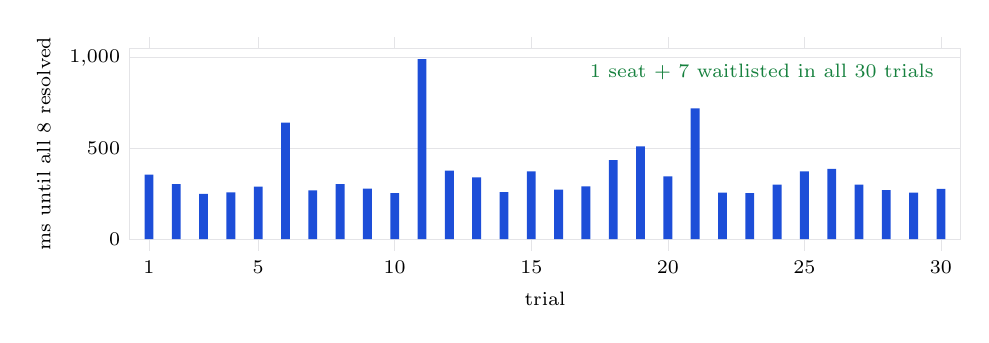
\begin{tikzpicture}
\begin{axis}[
  width=\columnwidth, height=4.0cm, ybar, bar width=3.2pt,
  xmin=0.3, xmax=30.7, ymin=0, ymax=1050,
  xlabel={trial}, ylabel={ms until all 8 resolved},
  xtick={1,5,10,15,20,25,30},
  tick label style={font=\scriptsize}, label style={font=\scriptsize},
  axis line style={line}, tick style={line}, major grid style={line}, ymajorgrids]
\addplot[fill=accent,draw=none] coordinates {
(1,355)(2,303)(3,250)(4,258)(5,289)(6,642)(7,269)(8,303)(9,278)(10,254)(11,992)(12,378)(13,341)(14,259)(15,373)
(16,273)(17,291)(18,435)(19,511)(20,346)(21,721)(22,256)(23,253)(24,301)(25,373)(26,388)(27,301)(28,270)(29,257)(30,277)};
\node[font=\scriptsize,okgreen,anchor=north east] at (rel axis cs:0.98,0.97) {1 seat + 7 waitlisted in all 30 trials};
\end{axis}
\end{tikzpicture}
\caption{Eight-way races for the last seat. The row lock serialises claimants; the outcome was correct every time.}
\label{fig:race}
\end{figure}

\subsection{Latency}
Figure~\ref{fig:lat} shows server-side latency per operation as seen by the client, including Limbo's database work and
the round trip to Nexconn. Posting a verified update (validate, store, sign, send through Nexconn) takes a median
94\,ms. Pool creation is the slowest operation because it also creates a Nexconn group channel. Reading room state
from Postgres takes under 10\,ms. A fact or confirmation posted in one browser appears in another in about a second.

\begin{figure}[t]
\centering
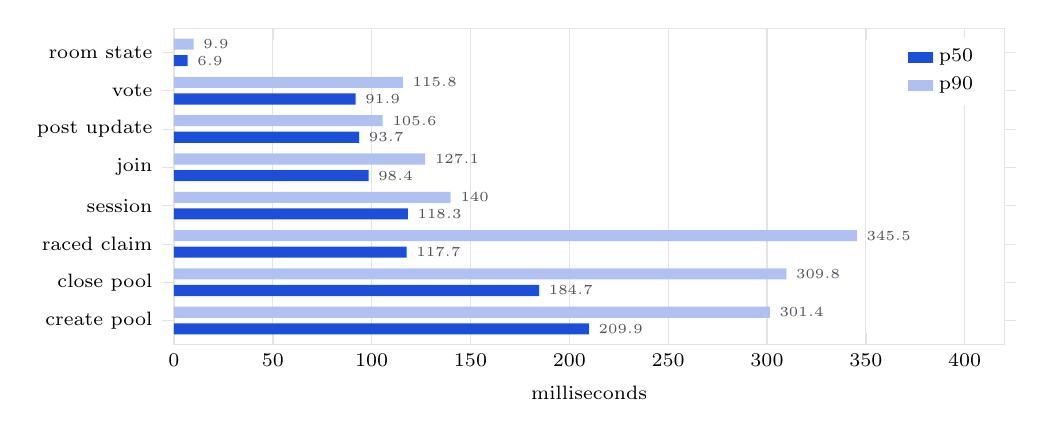
\begin{tikzpicture}
\begin{axis}[
  width=\columnwidth, height=5.6cm, xbar, bar width=4pt,
  xmin=0, xmax=420, xlabel={milliseconds},
  symbolic y coords={room state,vote,post update,join,session,raced claim,close pool,create pool},
  ytick=data, y dir=reverse, enlarge y limits=0.09,
  tick label style={font=\scriptsize}, label style={font=\scriptsize},
  axis line style={line}, tick style={line}, major grid style={line}, xmajorgrids,
  legend style={font=\scriptsize,draw=none,at={(0.98,0.97)},anchor=north east}, legend cell align=left,
  legend image code/.code={\fill[#1] (0cm,-0.07cm) rectangle (0.32cm,0.07cm);},
  nodes near coords, every node near coord/.append style={font=\tiny,text=ink2}, nodes near coords align={horizontal}]
\addplot[fill=accent,draw=none] coordinates {(6.9,room state)(91.9,vote)(93.7,post update)(98.4,join)(118.3,session)(117.7,raced claim)(184.7,close pool)(209.9,create pool)};
\addplot[fill=accent!35,draw=none] coordinates {(9.9,room state)(115.8,vote)(105.6,post update)(127.1,join)(140,session)(345.5,raced claim)(309.8,close pool)(301.4,create pool)};
\legend{p50,p90}
\end{axis}
\end{tikzpicture}
\caption{Server latency per operation (34 guests, 30 races; \code{npm run bench}).}
\label{fig:lat}
\end{figure}

\subsection{Resilience and weight}
With the connection cut, the offline notice appears in under 0.1\,s (Limbo listens to the browser's own network events
rather than waiting for the SDK's next heartbeat, which took over 40\,s). After reconnecting, the client pages through
history and refreshes signed state; across 11 runs it caught up on the missed message and update in a median
\textbf{0.8\,s} (range 0.2--1.3\,s). The room page ships 239\,KB of gzipped JavaScript (most of it the Nexconn SDK),
6\,KB of CSS and 3\,KB of HTML.

\begin{table}[h]
\centering\small
\caption{Code size (non-blank lines).}
\label{tab:loc}
\begin{tabular}{@{}lr@{\hspace{1.4em}}lr@{}}
\toprule
UI components & 2{,}266 & Server logic & 1{,}165 \\
Client logic & 879 & Shared logic & 655 \\
Pages & 401 & API routes & 302 \\
Tests and bench & 662 & SQL (12 tables) & 121 \\
\bottomrule
\end{tabular}
\end{table}

\subsection{Bugs found by testing}
Using the app as real people found problems that reading the code did not: Ed25519 missing in older Chrome (every card
vanished), actions reachable only on hover (unusable on phones), a 40-second delay before the offline notice, a
sessions limit that would lock out a whole airport sharing one IP address, a single failed Nexconn request failing a
user's action (now primary, backup, then primary again), and a people count that did not change when someone joined.
All are fixed and covered by tests.

% ------------------------------------------------------------------ 9
\section{Business model}\label{sec:biz}
Limbo is free for travellers, with no ads in the conversation. It is paid for by organisations that want calmer,
better-informed passengers (Table~\ref{tab:biz}). Growth is built in: every room has a link and a printable QR poster
for the gate, each shared cab pulls in strangers, and disruptions are seasonal (winter fog in North India, monsoon,
holiday peaks), so the same routes fill rooms again every year.

\begin{table}[t]
\centering\small
\caption{Who pays.}
\label{tab:biz}
\begin{tabularx}{\columnwidth}{@{}>{\raggedright\arraybackslash}p{2.3cm} X >{\raggedright\arraybackslash}p{1.7cm}@{}}
\toprule
\textbf{Customer} & \textbf{Value} & \textbf{Model} \\
\midrule
Airlines, railways & One verified voice in every affected room, in every language; fewer people at the desk & Per carrier or per disruption \\
Airports, stations & Official updates per terminal; live view of where crowds are stuck & Annual licence \\
Travel agencies & Coordinated rebooking for customers on a cancelled trip & Per seat \\
Cabs, hotels & Labelled offers to people stuck right now & Per lead \\
Insurers & Aggregate disruption evidence; claims guidance & Partnership \\
\bottomrule
\end{tabularx}
\end{table}

\paragraph{Cost to run.} Nexconn bills by monthly active users. The challenge's Free Chat Plan covers 10{,}000 MAU for
a year at no cost; at 25{,}000 and 100{,}000 MAU the Pro plan costs \$1{,}960 and \$7{,}160 a month. Translation beyond
the free allowance costs \$0.02 per 1{,}000 characters. Hosting and database fit in free tiers at launch.

\paragraph{Value to Nexconn.} Each disruption brings hundreds of active chat users in a burst; verified staff bring
organisations onto the platform; and a single room exercises community channels, group channels, custom messages,
metadata, history, translation and the Server API.

\paragraph{Traction.} Usage is measured from real rooms only (demo rooms and simulated users are excluded) on a private
dashboard: real users, rooms used, rooms with two or more people, updates, votes, pools, seats claimed, returning
users and daily actives. The same totals are public and live at \href{https://limbo-sooty.vercel.app/traction}{\code{limbo-sooty.vercel.app/traction}}.

% ------------------------------------------------------------------ 10
\section{Limitations and future work}
Signing proves that the server said something, not that the crowd is right; Limbo cannot verify a rumour, only show how
well-supported it is and let it fade. Staff verification is manual. Trip codes are not checked against live schedules,
so a mistyped code opens a separate room (mitigated by confirmation prompts). Translation is bounded by the free quota.
Next steps are schedule data to validate codes and seed rooms with official status, push notifications for room
updates through Nexconn, an operator console for verified staff, and per-terminal views for airports.

% ------------------------------------------------------------------ 11
\section{Conclusion}
A trip number is a meeting place that everyone affected already knows. Limbo turns it into a room on Nexconn that
exists before anyone joins, adds a board that the crowd confirms and nobody can forge, and lets strangers share the cost
of getting home, fairly. It is tested end to end against a live Nexconn app, and it is free for the people who need it
most: everyone stuck at the same gate.



\appendix
\section{Reproducing the results}
\begin{small}
\begin{verbatim}
cp .env.example .env.local   # App Key, App Secret, secrets
createdb limbo && npm install
npm run db:migrate
npm run build && npm start
npm test                     # 20 unit tests
npm run e2e                  # 58 end-to-end checks
npm run bench                # races and latency
\end{verbatim}
\end{small}
Nexconn console settings required: community channel cloud retention, pre-join history, and translation.

\end{document}
